\section{From model to simulation}
\label{sec:model-to-simulation}
In this section we outline the additional assumptions and methods that are 
needed to turn the model as described in section~\ref{sec:the-model} into a 
numerical simulation on a computer. This includes clearing up ambiguities and 
filling in gaps in the model definition.  The goal is, of course, to actually 
create a working simulation of the model.  Some of the components described in 
this section we have come up with ourselves, and others we have collected from 
various other publications related to social force models. References are 
noted where applicable.

The questions we resolve in this section are how to approximate the movement 
of pedestrians, how to set initial conditions and constants and how to 
identify the points on the walls to calculate repulsion from. Approximation of 
the movement is needed when turning the model into a concrete numerical 
simulation. Initial conditions are needed to set up the simulation, but not 
all parameters are given in the articles. Finally, as it is noted in 
section~\ref{sec:wall-repulsion}, in some geometrical cases, there are some 
ambiguities that become apparent when determining which points to use in the 
calculation of the repulsion from the walls. These problems are discussed in 
the following sections.

\subsection{Approximating continuous movement}
\label{sec:continuous-movement}
The model can be viewed as representing $4n$ coupled differential 
equations, where $n$ is the number of pedestrians. These differential 
equations describe the positions and speed of movement of the pedestrians in 
the $x$ and $y$ directions. Since we cannot solve these equations 
analytically, we will approximate them by doing numerical simulations in 
discrete time steps. There are various ways of approximating differential 
equations such as those represented by the model; we have chosen to use 
Euler's method as it is simple to work with. Euler's method is given by a 
truncated Taylor expansion \cite{MD}:

\begin{equation}
    p(t+\Delta t)=p(t)+V(t)\Delta t + \frac{1}{2}f(t)\Delta t^2
\end{equation}     

Here $p$ is the position, $V$ is the velocity, $f$ is the total force and $\Delta t$ 
is the time step. Similar we have the velocity given as:

\begin{equation}
    V(t+\Delta t)=V(t)+f(t)\Delta t
\end{equation}    

Euler's method, while simple, is not a very precise way of estimating the 
equations, and is very sensitive to choosing a suitable time step. Various 
more advanced methods of choosing the time step size as well as better 
algorithms to estimate the equations exist \cite{MD}. However, these methods 
are much more complicated to work with for a model as complex as ours. Since 
Euler's method is specifically mentioned as method used in \cite{ABconstant}, 
we have chosen to stick with this method despite its disadvantages.

\subsubsection{Choosing the time step}
\label{sec:choosing-timestep}
Choosing a suitable time step size is important when applying Euler's method.  
There are two main trade-offs in selecting this step size: precision of the 
approximation and numerical rounding errors. If the step size is too large, 
Euler's method will yield an approximation that differ too much from the 
actual values of the equations. In our case this would result in pedestrians 
changing direction and velocity too slowly, making them e.g. move through a 
wall between two time steps. However, lowering the time step size will, apart 
from resulting in longer calculation times, potentially increase the error 
introduced by rounding errors. Rounding errors occur because numerical 
simulations have a finite precision and so have to be truncated. The more 
calculations occur, the larger this error becomes. This means that setting the 
time step too low will result in too many errors from this source \cite{RoundingError}.

Methods for obtaining better approximations of differential equations exist, 
e.g. the Runge-Kutta method \cite{butcher2003}. However, from experimenting 
with various time step values, we have found that using Euler's method and 
setting a suitably small static time step provides reasonable results, so we 
have chosen not to complicate our simulation further by applying more advanced 
methods.

\subsection{Initial conditions and constants}
\label{sec:init-cond}
As seen in section~\ref{sec:the-model}, there are various parameters that must 
be set in order to simulate the model. Apart from this, there are also various 
initial conditions (such as the pedestrians' starting position) that must be 
set. In this section, we outline these parameters and initial conditions, 
describe how we have obtained their values and how we plan to vary them 
when we run the simulations.

\subsubsection{A note on random numbers}
Some of the initial conditions are set using random distributions, either 
uniformly or Gaussian distributed, in order to simulate national variations in 
e.g. the radius of pedestrians.  These random numbers are created by the 
pseudorandom number generator built in to the Python programming language.  
This generator is an implementation of the Mersenne twister 
generator\footnote{See \url{http://en.wikipedia.org/wiki/Mersenne\_twister}} 
and we consider it sufficient for our purposes. This type of pseudorandom 
number generator is deterministic for identical seed values, which means we 
can run multiple simulations of the same initial conditions by fixing the seed 
of the random number generator to the same value for each run.

Of course the use of (pseudo)random numbers may be a source of errors. We 
discuss this further in section~\ref{sec:random-errors}.

For the initial conditions that are Gaussian distributed, we obtain 
distributions by using the distribution functions of the \emph{NumPy} 
mathematical library for Python \cite{numpy}.

\subsubsection{Scenario geometry}
We set various parameters that describe the geometry of the scenarios we want 
to simulate. We have defined these ourselves, from the scenario descriptions 
given in section~\ref{sec:results}. These parameters are:

\begin{itemize}
    \item \textbf{Placement of walls:} The placement of the walls is described 
        by defining the endpoints describing the line segments that 
        constitute each wall.

    \item \textbf{Pedestrian starting areas:} For each scenario we define one 
        or more areas in which the pedestrians start. The pedestrians are 
        distributed randomly within these areas, as described below.

    \item \textbf{Pedestrian targets:}  Pedestrians move toward their 
        assigned target, as described in section~\ref{sec:desired-force}. 
        Targets do not differ between pedestrians, except that we assign a 
        target for each starting area to allow for simulating scenarios where 
        pedestrians move towards each other in groups.

        Since the model does not deal with path finding, targets are not 
        changed during the simulation. When a pedestrian reaches its target, 
        it is considered to have escaped, and is removed from the simulation.
\end{itemize}


\subsubsection{Pedestrians' parameters}
\label{sec:init-pedestrians}
There are a number of parameters that relate to the pedestrians. They are:

\begin{itemize}
    \item \textbf{Pedestrians' radii:} The radii of the pedestrians, 
        $R_\alpha$, is drawn from a Gaussian distribution with a mean of $0,3$ 
        meters and a standard deviation of $0,05$ meters. This is done to 
        simulate a natural variety in the width of human shoulders, and to 
        avoid deadlocks caused by perfectly symmetrical forces that might 
        otherwise occur. This method of assigning pedestrian radii is taken 
        from \cite{self-org}.
        %TODO: Check source.
        
    \item \textbf{Pedestrian positions:} Pedestrians start out randomly 
        distributed throughout the designated starting areas defined for each 
        scenario. We have not found an explanation for how this is done in any 
        of the articles, so we have come up with the following algorithm for 
        placing pedestrians:

        To avoid having pedestrians start out on top of each other, the 
        starting area is divided into a grid with cells a little larger than 
        the size of the maximum diameter of the generated pedestrians. The 
        pedestrians are then placed into random cells of the grid. This makes 
        the starting configuration of the pedestrians a little more rigid than 
        what might otherwise be observed, but we feel this is acceptable since 
        pedestrians move out of these grid cells within the first few time 
        steps.
        
    \item \textbf{Initial velocity:} As described in 
        section~\ref{sec:desired-force}, the initial pedestrian velocity is 
        assumed to be zero.


    \item \textbf{Initial desired speed:} The initial desired speed, 
        $V^{Id}_\alpha$, for the pedestrians is set to be Gaussian 
        distributed with a mean of $1,3$ and a standard deviation of $0,3$.
	These values are taken from \cite{self-org}. 


    \item \textbf{Maximum desired speed :} The maximum desired speed is set to 
        $V_{\alpha}^{max}=1,3V^{Id}_\alpha$.
	As the initial desired speed this value is also taken from \cite{social-force}.
      
        
    \item \textbf{Relaxation time:} The relaxation time, $\tau$, is set to $1$ 
        second in \cite{self-org}. 
\end{itemize}

\subsubsection{Constants} \label{constants}
The model includes a number of constants. These are parameters that do not 
vary between the pedestrians, but are fixed for the whole simulation. They are:

\begin{itemize}
    \item \textbf{Time step size:} We have experimented with various time step 
        sizes, and have found that with a fixed value of $0.01$ seconds, we 
        get reasonable results from our simulation.

    \item \textbf{$A$, $B$:} We set $A=3.0$ and $B=0.2$, taken from  
        \cite{self-org}.

    \item \textbf{$U$:} Is not given in \cite{self-org} so instead we have taken 
 			it from \cite{social-force} where they set $U$ to be $10.0 m^2 s^{-2}$.

    \item \textbf{$\lambda$:} We set $\lambda=0.75$, from 
            \cite{self-org}.
\end{itemize}

\subsubsection{Varying the parameters}
\label{sec:varying-constants}
A way of analysing the behaviour of the model would be to systematically vary 
the different parameters to assess how this affects model behaviour and to 
find out which parameter values makes the model break down. However, since we 
have several parameters that could be varied (11 in total, not counting the 
scenario geometry), it is impractical to do this manually. Doing it 
automatically would require us to develop measures of simulation viability 
that can be measured automatically; and since our assessment of which 
simulations are useful very much rely on visual inspection (e.g. if actors 
walk through walls a simulation is considered invalid), we would have to come 
up with an exhaustive set of tests that would tell us whether or not 
simulations are valid. Our cursory testing of arbitrarily chosen parameter 
values indicates that there are several ways in which simulations can be 
invalid, so we have deemed it out of scope of this project to develop such 
tests, and so we have chosen instead to abandon the attempt to do systematic 
parameter variations.

Instead, we have started running our simulations using the parameter values 
outlined above, and then only vary parameters when these values do not work. 
While this does not give us an exhaustive overview of the model behaviour, it 
is sufficient to test whether or not we see the phenomena we are trying to 
reproduce.

\subsection{Finding the nearest point on a wall}
\label{sec:repulsion-points}
As mentioned in section~\ref{sec:wall-repulsion}, it is not clear from the 
article how the nearest point $p_{\gamma \alpha}$ on a wall from a given 
pedestrian is found. In many cases it is obvious: $p_{\gamma \alpha}$ is the 
point of intersection of the wall and a line perpendicular to the wall passing 
through $p_\alpha$ (the projection of $p_\alpha$ onto the wall).

However, since walls are described as line segments, such a point is not 
guaranteed to exist; the pedestrian may be positioned off either end of the 
wall. In the simple case, this is easily remedied: simply define $p_{\gamma 
\alpha}$ as the projection of $p_\alpha$ onto the wall, and if no such 
projection exists, define $p_{\gamma \alpha}$ to be the wall endpoint closest 
to $p_\alpha$. This approach works except for two cases: When walls have kinks 
and at doorways.

\subsubsection{Walls with kinks}
Since each wall is defined as a line segment, a single wall cannot have kinks 
in it. To define such a wall, multiple line segments are defined with shared 
end points. When the angle between such two walls is greater than $180^\circ$, 
as indicated by the angle $\theta$ in figure~\ref{fig:wall-kinks}, a 
problem appears.

The reason for this problem is that the same endpoint may be indicated for 
repulsion from multiple walls. Looking at figure~\ref{fig:wall-kinks}, a 
pedestrian in area A will be repulsed both by a point on the wall $\gamma_1$, 
but also from the nearest endpoint of $\gamma_2$, which is shared with 
$\gamma_1$. A pedestrian in area B will be repulsed from both walls at the 
endpoint shared between $\gamma_1$ and $\gamma_2$. Both these situations will 
result in an extra repulsion that is the result of the way walls are 
represented (as line segments), and not a part of the model. To avoid this, 
the algorithm in \ref{sec:repulsion-points-algorithm} for selecting which points 
to calculate wall repulsion from has to take this into account.

\begin{figure}[h]
    \centering
    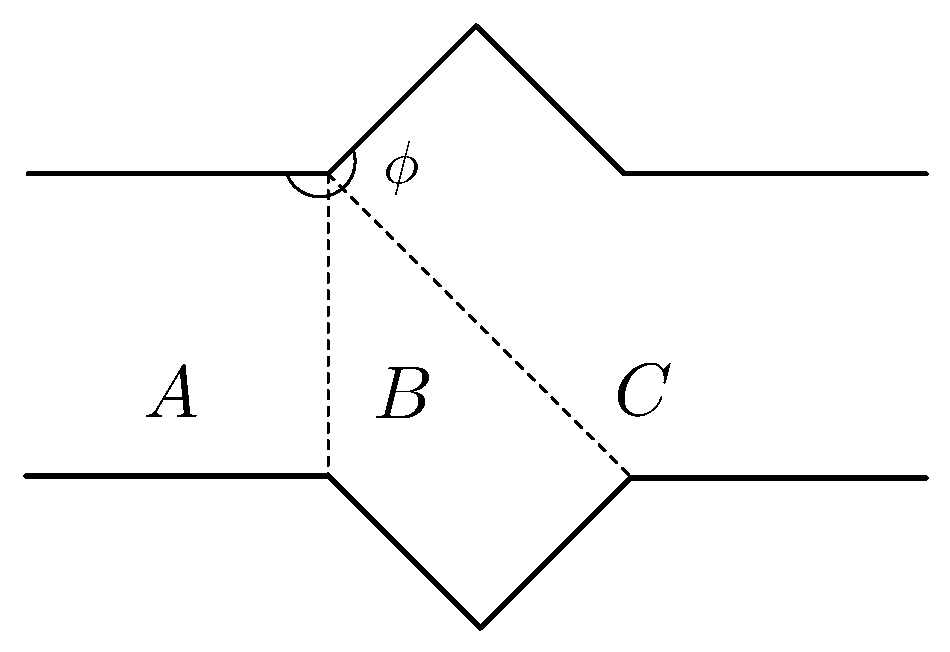
\includegraphics[scale=0.45]{Figures/WallCase.pdf} \caption[A wall with 
    kinks]{A wall with kinks. A pedestrian $\alpha$ in the area A will be 
    repulsed by a point on the wall $\gamma_1$ and by the nearest endpoint of 
    $\gamma_2$. In the area B, $\alpha$ will be repulsed twice by the endpoint 
    shared between $\gamma_1$ and $\gamma_2$. This situation occurs when the 
    angle $\theta > 180^\circ$.}
    \label{fig:wall-kinks}
\end{figure}

\subsubsection{Doorways}
Another problem occurs at doorways: if the wall repulsion points are set to be 
the nearest endpoints of wall segments, a pedestrian passing through a doorway 
would be repulsed by both sides of this doorway, creating an unwanted barrier 
for passing through it. In simulations, this appears as a force 
that pedestrians have to overcome to escape through doorways.

To solve this problem, the algorithm for selecting which points on the walls 
to calculate the repulsion from must take into account that once a pedestrian 
is passing through a doorway, no repulsion should be calculated from the wall 
segments that form the door. A way to accomplish this is to distinguish 
between endpoints that are shared with other walls, and endpoints that are 
``free-floating''. Such endpoints are only considered for repulsion if they 
are closer to the pedestrian than its radius, i.e. if the pedestrian touches 
the wall. This is illustrated in figure~\ref{fig:doorways}.

\begin{figure}[h]
    \centering
    \begin{tikzpicture}
		\node (p)  [pedestrian] {};
		\node (left endpoint) [wall endpoint,above left=3mm of p] {};
		\node (right endpoint) [wall endpoint,right=of left endpoint] {};
        \node (target) [point,above right=of left endpoint] {};

        \node (top l) [point, left=of left endpoint] {};
        \node (top r) [point, right=of right endpoint] {};
        \node (bottom l) [point, below=3cm of top l] {};
        \node (bottom r) [point, below=3cm of top r] {};

        \draw [wall,name path=wall] (left endpoint) -- (top l) -- (bottom l) 
            -- (bottom r) -- (top r) -- (right endpoint);

        \path [name path=dotted l] (left endpoint) -- +(0,-3.1);
        \path [name path=dotted r] (right endpoint) -- +(0,-3.1);
        \path [name intersections={of=wall and dotted l, by=dot 1}];
        \path [name intersections={of=wall and dotted r, by=dot r}];

        \draw [dotted] 
                (left endpoint) ++(0,0.5) -- (dot 1) 
                (right endpoint) ++(0,0.5) -- (dot r);

        \draw [distance marker] (p.center) -- (left endpoint);
		\draw [vector] (p) -- (target);
    \end{tikzpicture}

    \caption[Preventing repulsion from doorways]{Preventing repulsion from 
    doorways. To allow free passage for pedestrians between the 
    dotted lines. This means that the pedestrian do not get repulsed from the marked endpoints unless the 
    distance (indicated by the dashed line) is smaller than the pedestrian's 
    radius.}
    \label{fig:doorways}
\end{figure}

\subsubsection{Algorithm for identifying wall repulsion points}
\label{sec:repulsion-points-algorithm}
Based on the description above, we have devised the following algorithm for 
selecting which points on the walls should be included when calculating the 
repulsion force from walls.

The algorithm is run for each pedestrian. Its input is the pedestrians 
position, $p_\alpha$ and the set of starting points and endpoints of the 
walls. The output is the set of points from which repulsion should be calculated. A 
set of endpoints that are already used and endpoints that are candidates for 
repulsion are used during the operation of the algorithm.

\begin{enumerate}
    \item For each wall, calculate the projection of the vector pointing from 
        the wall's starting point to the pedestrian, unto the vector pointing 
        from the wall's starting point to its endpoint.
        \begin{enumerate}
            \item If this point is part of the wall, add it to the set of 
                points repulsion should be calculated from, and add the wall's 
                two endpoints to the set of already used endpoints.

            \item If the projected point is not part of the wall, the endpoint closest 
                to the pedestrian is used instead. This endpoint is added to 
                the set endpoints that are candidates for repulsion.
        \end{enumerate}

    \item After having gone through all walls, for each point in the set of 
        candidate endpoints, check if this point is already in the set of 
        used endpoints. If it is, discard it. 

    \item Otherwise, check if the endpoint is shared with another wall (i.e. 
        if it appears twice in the set of candidate endpoints).
        
    \item If the endpoint is either shared with another wall or closer to the 
        pedestrian than the pedestrian's radius, add it to the set of 
        repulsion points.
\end{enumerate}

Our implementation of this algorithm is described in 
section~\ref{sec:model-calculation}.

\subsection{Summary}
In this section we have discussed the things that are needed to turn the model 
description into a numerical simulation. These things are approximating the 
movement of pedestrians through Euler's method, setting initial constants and 
parameters, and an algorithm for identifying the points on the walls nearest 
to a pedestrian. Some of the solutions to the problems associated with turning 
the model into a simulation we have found solutions of in the literature, and 
some we have come up with ourselves. Euler's method and some of the constants 
belong in the former group, while other constants and the algorithm for 
identifying wall points belong in the latter.

In the following section, we outline how we have implemented our simulation.
